\section{The claim and the short answer}\label{sec:claim}

\textbf{The claim (yours).} A model of a given size can hold the meaning of only so many words.
A small vocabulary needs only a small model. A larger vocabulary at the same model size does
worse.

\textbf{What was done.} A toy world of creatures and facts about them was made. Small models
were trained to know the facts, with 16 up to 1,024 creatures, with five sizes of model, and
with 8, 16, 32 and 64 bits to know about each creature. Every model was then graded on four
scores. The rules for judging the claim were written down before the first run.

\begin{keybox}
\textbf{Short answer.}
\begin{itemize}
\item \textbf{8 bits per creature: the claim was contradicted.} Every one of the \N{runs.main8}
  counted runs ended with every fact known (\N{main8.facts.lowest} or more out of 100).
  Models with \N{main8.c16.b8.equal.params.middle} trained numbers in the middle parts knew the
  facts of 1,024 creatures as well as those of 16. By the rule fixed beforehand, the verdict is
  \textbf{\N{verdict.overall}} (equal use: \N{verdict.equal}; unequal use: \N{verdict.zipf}).
  P1 \N{p1.equal.result}, P2 \N{p2.equal.result}, P3 \N{p3.equal.result}, P4
  \N{p4.equal.result}, the same for both kinds of use.
\item \textbf{What did change with more creatures:} the learning took longer (figure
  \ref{fig:speed}). Each new word also brings its own row of \N{rule.columns} trained numbers,
  so the model grows with the vocabulary (figure \ref{fig:params}). This report does not prove
  that this is the reason.
\item \textbf{With more bits per creature, larger vocabularies did score lower, but only at 64
  bits.} At 16 and 32 bits every setting ended with a median of \N{bits32.facts.lowest} facts known or more.
  At 64 bits, \N{below95.bits64} of \N{settings.bits64} settings ended below \N{rule.held}, as low as
  \N{bits64.facts.lowest}, and a bigger body helped only a little (section \ref{sec:bits}). The agent's
  expectation that failure would follow the bits and the body width, and not the number of creatures, was
  wrong there. Questions and ``not'' known fell earlier and further than facts known.
\item \textbf{Some scores were still rising when training stopped} (all \N{below95.rising.bits64} settings below \N{rule.held}). For those, the report
  cannot tell ``cannot hold'' from ``not learned yet'', because the longer control run
  was not done.
\end{itemize}
\end{keybox}

\textbf{How to read every picture.} Scores run from 0 to 100, and 100 means everything right.
A \emph{repeat} is the same setting trained again from new random starting numbers. A dot is one
repeat. A line joins the middle values (the median) of the repeats. Colour tells the size of the
model, or the number of creatures, and each figure says which.

\section{What was wrong with the first experiment, and what changed}\label{sec:changes}

\begin{center}\small
\begin{tabularx}{\textwidth}{@{}>{\raggedright\arraybackslash}p{0.33\textwidth}X@{}}
\toprule
First experiment & This experiment\\
\midrule
``Width'' changed the length of every word's row and the size of the middle parts together
& Every word has a row of \N{rule.columns} numbers in every run. Model size is only the
neurons in the middle part of each layer (body width: 8, 16, 32, 64 or 128)\\
20 sentences per animal, each read thousands of times
& Sentences about up to four creatures at once, new almost every time. Billions of true lines
of text exist (section \ref{sec:language})\\
About ten sentences in one row, so a model could look back at an earlier one
& One line of text per row\\
Runs stopped when they looked flat, which proved unreliable
& Every run has the same fixed length, set beforehand from practice runs\\
3 repeats, and 1 for most of the harder round
& Counted stages have \N{rule.repeats} repeats (8 bits), 3 (16 and 32 bits) and 2 (64 bits)\\
Scored on sentences it had read
& Also scored on creature pairs it has never read together\\
More bits came with season words, a different kind of sentence
& More bits come as more kinds of fact, in the same kind of sentence\\
\bottomrule
\end{tabularx}
\end{center}

The word table was a decision of yours on 22 November, made before any run. In ordinary models
every word has a row of numbers in a table and the table is trained along with the rest. The
first experiment did that, and so does this one. A table that is \emph{frozen} (never trained)
exists as a switch. It was \textbf{not run}.

\section{The language}\label{sec:language}

The world has creatures and facts about them. The creatures have the same names as in the first
experiment (\s{foxes}, \s{bears}, \s{wolves}, \s{owls}, \ldots, up to 1,024 names). A run uses
the first 16, 64, 256 or 1,024 of them.

Each creature has one value for each \emph{kind of fact}. A kind has a linking phrase and four
possible values. Four values are 2 bits. So 4 kinds are 8 bits per creature, 8 kinds are 16
bits, 16 kinds are 32 bits and 32 kinds are 64 bits. The first kinds are:

\begin{center}\small
\begin{tabular}{@{}lll@{\qquad}lll@{}}
\toprule
Kind & Phrase & Values & Kind & Phrase & Values\\
\midrule
1 & \s{are} & \s{red brown green black} & 3 & \s{live in} & \s{woods fields rivers caves}\\
2 & \s{eat} & \s{meat plants insects seeds} & 4 & \s{wake at} & \s{dawn noon dusk night}\\
\bottomrule
\end{tabular}
\end{center}

Kinds 5 to 32 have the same shape, with their own phrases and four values each (for example
\s{fear}, \s{like} and \s{carry}). Exactly a quarter of the creatures have each
value of a kind. A random shuffle that is the same in every run decides which.

\textbf{Lines of text.} A line speaks about one to four creatures, and ends at the full stop or
the answer. The longest line has 13 words. The model only ever reads true lines. For example (the
facts here are real ones of the 16-creature language):

\begin{itemize}
\item A statement: \s{toads and wolves eat insects .}
\item A ``not'' statement: \s{otters , crows and bears do not wake at night .}
\item A question with its answer: \s{do wolves , frogs and lizards wake at night ? yes}
\item A question answered ``no'': \s{do ducks eat insects ? no}
\end{itemize}

A statement about several creatures is true when every one of them has the value. A ``not''
statement is true when none of them has it. A question is answered \s{yes} when every creature
in the list has the value, and \s{no} otherwise.

\textbf{How many valid lines.} Counting lists in a different order as different lines, and not
yet taking away the lines that hold a held-back pair (next section), the language has this many
true lines:

\begin{center}\small
\begin{tabular}{@{}rrrrr@{}}
\toprule
Bits per creature & 16 creatures & 64 creatures & 256 creatures & 1,024 creatures\\
\midrule
8 (4 kinds)  & \N{lang.sentences.k4.c16} & \N{lang.sentences.k4.c64} & \N{lang.sentences.k4.c256} & \N{lang.sentences.k4.c1024}\\
16 (8 kinds) & \N{lang.sentences.k8.c16} & \N{lang.sentences.k8.c64} & \N{lang.sentences.k8.c256} & \N{lang.sentences.k8.c1024}\\
32 (16 kinds) & \N{lang.sentences.k16.c16} & \N{lang.sentences.k16.c64} & \N{lang.sentences.k16.c256} & \N{lang.sentences.k16.c1024}\\
64 (32 kinds) & \N{lang.sentences.k32.c16} & \N{lang.sentences.k32.c64} & \N{lang.sentences.k32.c256} & \N{lang.sentences.k32.c1024}\\
\bottomrule
\end{tabular}
\end{center}

A model reads \N{sentences.main8} lines in a 8-bit run, so with 16 creatures it sees many lines
more than once, and with 1,024 creatures almost none twice.

\textbf{Word use.} In \emph{equal use} every creature is mentioned equally often. In
\emph{unequal use} the second creature is mentioned half as often as the first, the third a
third as often, and so on. This is the rule of the first experiment. Real languages look roughly
like this.

\section{The model}\label{sec:model}

The model is a small transformer, built like the one in the first experiment. It reads a line one
word at a time and, at every place, guesses the next word. It has two layers. Each layer has an
attention part and a \emph{middle part}. The middle part is a small network: \N{rule.columns}
numbers go in, a layer of neurons follows, and \N{rule.columns} numbers come out. The number of
neurons in that layer is the \emph{body width}: 8, 16, 32, 64 or 128. It is the size of the
model in this experiment. This report says ``neurons in the middle part of each layer'' or ``body
width''. With body width 8 the middle parts hold \N{main8.c16.b8.equal.params.middle} trained
numbers, and with body width 128 they hold \N{main8.c16.b128.equal.params.middle}.

\textbf{The word table, trained.} Each word is first turned into a row of \N{rule.columns}
numbers, read from the \emph{word table}. In every counted run this table is \textbf{trained}:
its numbers change during learning, like all the others. Every run starts from the same table.
Only words that are in use get any change. This has a consequence that matters for the claim:
\emph{every word in use brings its own row of \N{rule.columns} trained numbers}. With 16
creatures and body width 8 the model has \N{main8.c16.b8.equal.params.trained} trained numbers.
With 1,024 creatures and the same body width it has \N{main8.c1024.b8.equal.params.trained}
(figure \ref{fig:params}).

\textbf{What a frozen word table would mean.} The numbers would be drawn once at random and
never change. The model would then have to keep everything it knows about a creature in the
middle parts, because the creature's row could not adapt. Then a new word would bring no
storage of its own. That is the cleanest form of your claim. It is ready (stage
\texttt{frozen8}) and \textbf{was not run}.

The model never has to say a creature's name. Its output layer can only produce the other words.

\section{The test}\label{sec:exam}

After training, the model is graded on a fixed exam. All scores run from 0 to 100 and are made on
an averaged copy of the model, the one that is saved. There are four scores.

\begin{enumerate}[itemsep=1.5pt]
\item \textbf{Facts known} (the main score). For every creature and every kind, the model gets
  the start of a statement (\s{foxes are}) and must give the highest score to the right value
  among the four. Guessing gives 25.
\item \textbf{Questions about one creature.} For every creature and kind, one \s{yes} question
  with the true value and three \s{no} questions with the other values. The score is the share
  of \s{yes} right plus the share of \s{no} right, minus 100, and not below 0. Guessing gives 0.
\item \textbf{Questions about new combinations.} Questions about 2 to 4 creatures that include a
  pair that was never read together. Scored like the score above. Guessing gives 0.
\item \textbf{``not'' known.} For every creature and kind, the start of a ``not'' statement
  (\s{foxes are not}). Right when the true value gets the \emph{lowest} score of the four.
  Guessing gives 25.
\end{enumerate}

\textbf{Held-back pairs, with an example.} One tenth of all pairs of creatures are held back, at
random: \N{lang.held.c16} of the \N{lang.pairs.c16} pairs for 16 creatures. Suppose \s{foxes} and
\s{owls} are a held-back pair. Then no line the model reads has both in its list. It may read
``\s{foxes are red .}'' and ``\s{owls and bats eat seeds .}''. Later it is asked
``\s{do foxes and owls eat meat ? }'' and has to answer from what it knows of each alone. The
exam has up to 2,000 such questions: \N{qnew.count.c16} for 16 creatures, \N{qnew.count.c1024} for
1,024. The score on 16 creatures rests on few questions, so it is coarse.

\section{The predictions and the rule, fixed beforehand}\label{sec:rule}

Written down in the plan before any run. ``Facts known'' is read at the end of the fixed
training length. A prediction holds for a setting when it holds in at least \N{rule.needed} of
its \N{rule.repeats} repeats.

\begin{itemize}
\item \textbf{P1: a small vocabulary needs only a small model.} With 16 creatures every body
  width reaches \N{rule.held} or more.
\item \textbf{P2: a larger vocabulary at the same size does worse.} At body width 8, the score on
  1,024 creatures is at least \N{rule.gap} points below the score on 16 creatures.
\item \textbf{P3: a larger model holds more.} On 1,024 creatures, body width 128 scores at least
  \N{rule.gap} points above body width 8.
\item \textbf{P4: the agent's expectation, the opposite of P2.} With a trained word table the
  number of creatures makes little difference: at every body width the score on 1,024 creatures
  is within \N{rule.gap} points of the score on 16 creatures. The reason, given beforehand: each
  creature has its own row of \N{rule.columns} trained numbers, enough for its 8 bits, so a new
  word brings its own storage. \emph{If anything fails, the agent expects it to follow the bits
  per creature and the body width, not the number of creatures.}
\end{itemize}

P2 and P4 cannot both hold. The runs decide between them.

\textbf{The verdict.} The claim is \emph{supported} if P1, P2 and P3 hold, with equal use and with
unequal use. It is \emph{contradicted} if at every body width the score on 1,024 creatures is
within \N{rule.gap} points of the score on 16 creatures. Anything else is \emph{mixed}, and the
report says which parts held. The program that judges this was written before the results and
reads the rule so: P2 and P3 compare two settings repeat by repeat (same starting seed); ``within''
means a gap smaller than \N{rule.gap}; each kind of use is judged alone, and the overall verdict is
\emph{supported} or \emph{contradicted} only if both kinds agree.

\textbf{Held and not held.} For the stages with more bits no outcome was predicted, except the
last sentence of P4. A setting counts as ``held'' when facts known reaches \N{rule.held} in at
least \N{rule.needed} of 5 repeats (used for 8 bits). For other stages the report gives the median.

\section{How the settings were fixed (practice runs)}\label{sec:practice}

Two settings are not about the claim and had to be fixed first: the length of training and the
learning rate (how big each learning step is). They were set from practice runs with a starting
seed that is never used in counted runs (figure \ref{fig:practice}). The numbers of the plan are
repeated here from the result files.

\begin{figure}[H]
\centering
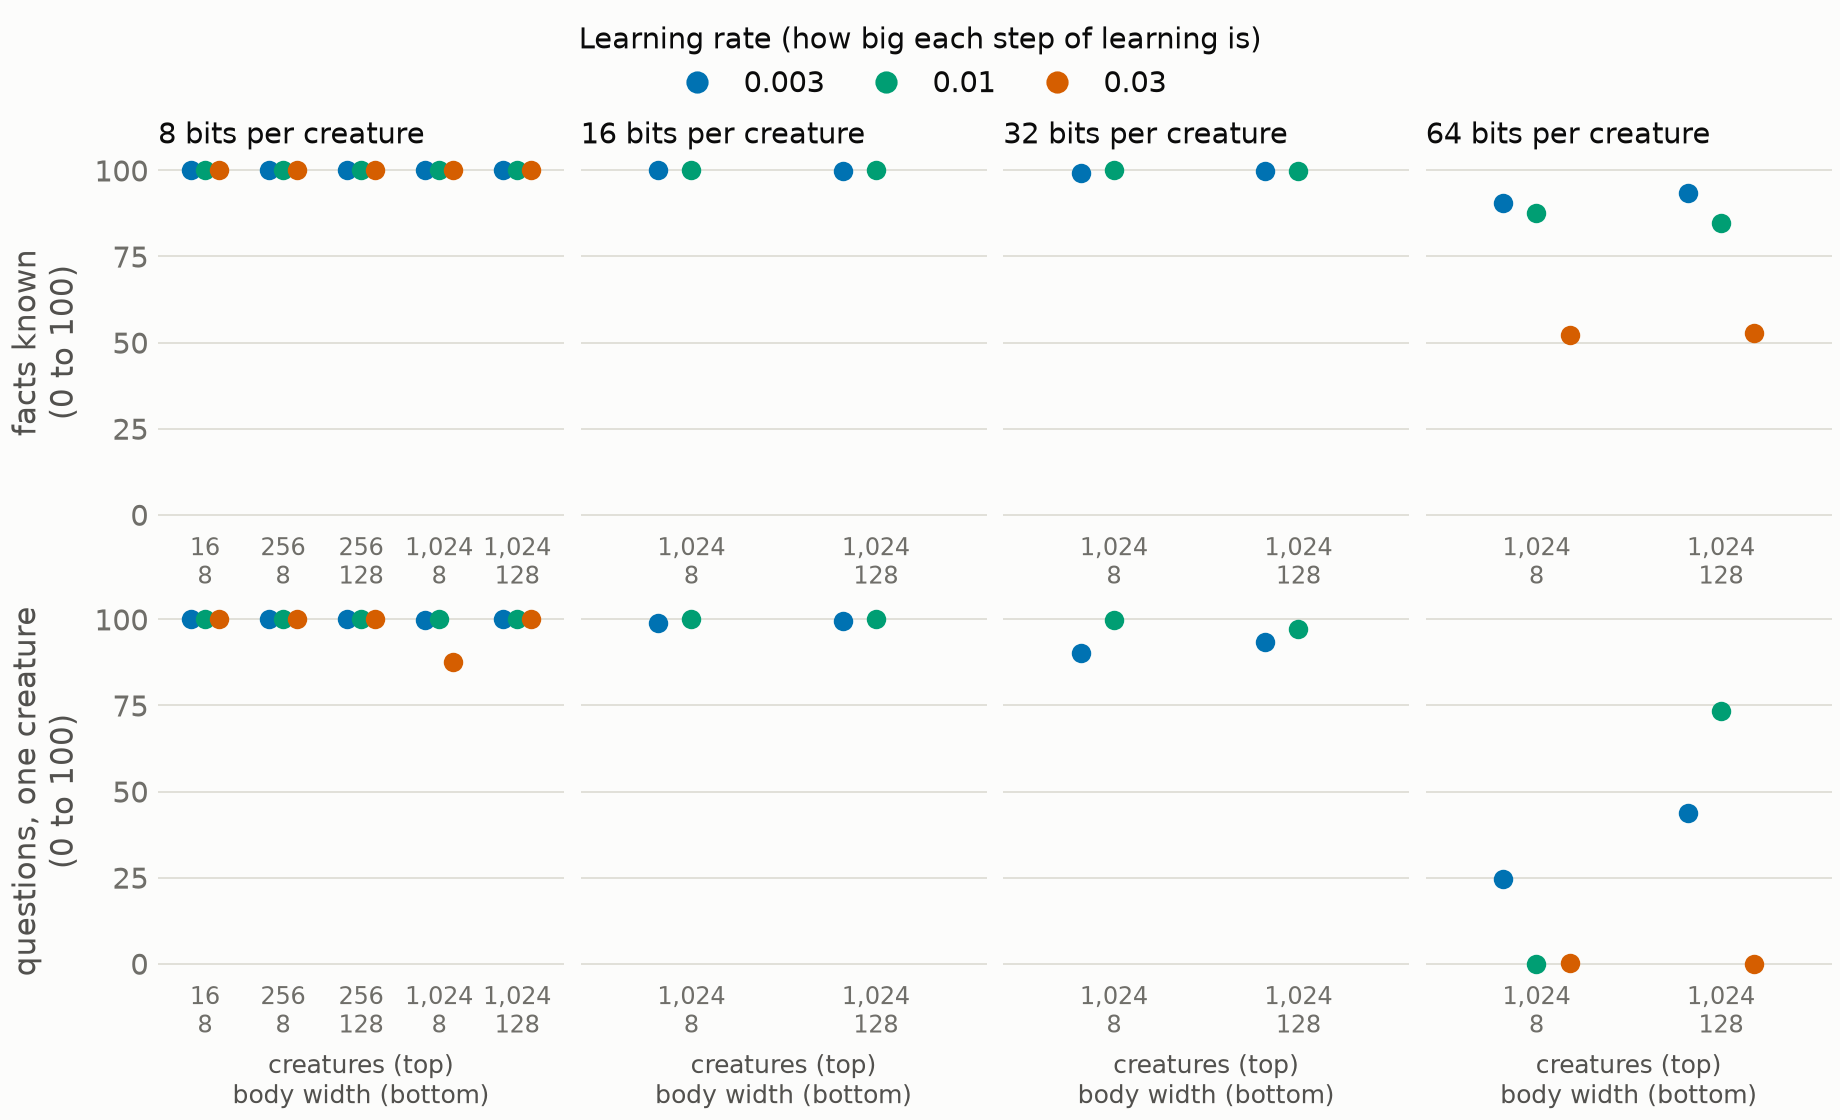
\includegraphics[width=0.88\textwidth]{figures/fig8_practice.png}
\caption{Practice runs. Each dot is one run (never counted) at the end of its training.}\label{fig:practice}
\end{figure}

\reads{fig:practice} Each panel is one number of bits per creature. Along the bottom of each panel
are the settings tried: the number of creatures on top, the body width below. The height of a dot
is the score at the end. The colour is the learning rate. Top row: facts known. Bottom row:
questions about one creature.

\shows{fig:practice} At 8 bits, every practice run knew all facts (for example
\N{pilot.k4.c1024.b8.lr0.03.facts} with rate 0.03 on 1,024 creatures and body width 8), but
a learning rate of 0.03 was worse on the questions (\N{pilot.k4.c1024.b8.lr0.03.q1} on 1,024
creatures with body width 8) and 0.003 was slower. At 64 bits, rate 0.003 reached the most facts
known (\N{pilot.k32.c1024.b8.lr0.003.facts} and \N{pilot.k32.c1024.b128.lr0.003.facts}), 0.01 was
lower (\N{pilot.k32.c1024.b8.lr0.01.facts} and \N{pilot.k32.c1024.b128.lr0.01.facts}) and 0.03 was
far lower (\N{pilot.k32.c1024.b8.lr0.03.facts} and \N{pilot.k32.c1024.b128.lr0.03.facts}).

\begin{itemize}
\item \textbf{8 bits.} Learning rate \N{lr.main8}, \N{steps.main8} steps of training for every
  run (\N{sentences.main8} lines read). The slowest practice run (1,024 creatures, body width 8, rate
  0.01, equal use) knew the facts (\N{rule.facts_goal}) by step \N{pilot.k4.c1024.b8.lr0.01.steps97}
  and the questions (\N{rule.questions_goal}) by step \N{pilot.k4.c1024.b8.lr0.01.steps90q}. No
  practice run used unequal use, where the rarest of 1,024 creatures turns up about \N{zipf.rarest.c1024} times less
  often than the average creature, so the length was set at about six times the slowest practice
  run. Fixed before any counted run.
\item \textbf{64 bits.} Learning rate \N{lr.bits64}, \N{steps.bits64} steps (\N{sentences.bits64}
  lines). The practice runs had not finished learning at \N{pilot.k32.c1024.b8.lr0.003.steps}
  steps, so the length is four times longer.
\item \textbf{16 and 32 bits.} Learning rate \N{lr.bits16} for both. \N{steps.bits16} steps for 16 bits
  and \N{steps.bits32} for 32 bits. At 32 bits the practice runs were still rising on questions
  about new combinations (\N{pilot2.k16.c1024.b8.lr0.01.qnew} and
  \N{pilot2.k16.c1024.b128.lr0.01.qnew}), so that length is one and a half times the practice length.
\end{itemize}
